\section{Background}
  In this section I will discuss the background work and research done for this project. I will start by disusing my teams place in the organisation and 
  our OKRs, explaining how this project helps us hit these objectives. I will then outline the current architecture and the initial design for the project.
  Finally I will discuss some areas of interest around project, these include cloud computing, database parallelisation strategies and CI/CD challenges.

  \subsection{Organisation}
  The BBC is broken into multiple layers with different responsibilities and goals. I am in a team called \textit{SpaceChimps} which is partner of
  the partnerships group, which itself is in the product group.

  \begin{figure}[H]
    \centering
    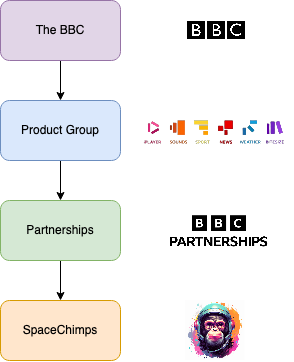
\includegraphics[width=4cm]{assets/bbcHierarchy.drawio.png}
    \caption{Image showing SpaceChimps place in the BBC (Bowker, 2023).}
    \label{fig:bbcHierarchy}
  \end{figure}

  Our main aim as a team is to provide data to partners that they can use on their devices to promote BBC content. The project described in this report does
  just that by providing schedules for live content to partners. This aim fits directly into Partnerships objectives:

  \begin{itemize}
    \item It helps drive growth as we are able to get content out to more people on more devices, increasing exposure to the BBC.
    \item It helps us improve our partner experience by working with them on integrating the data into their feeds.
    \item This project reduces the total time processing data, which therefore reduces our costs and makes us more sustainable.
  \end{itemize}

  All objectives can can be seen in \hyperref[sec:AppendixA]{\textbf{Appendix A}} (BBC Partnerships, 2023).

  \subsection{Current Architecture}
    \subsubsection{Initial design}

  \subsection{Research}
    \subsection{Cloud computing and microservices}
    \subsection{Database Parallelism}
    \subsection{CI/CD and it's challenges}

\newpage
